\documentclass[a4paper,openright,12pt]{article}
\usepackage[utf8]{inputenc}
\usepackage{graphicx} 
\usepackage{subfigure}
\usepackage[mathscr]{eucal}
\usepackage{titling}
\usepackage{float}
\usepackage{amsmath}
\usepackage{afterpage}
\usepackage{vmargin}
\usepackage[spanish]{babel}
\usepackage{eurosym} 
\usepackage{multirow} 
\usepackage{cite}
\usepackage{url}

\setpapersize{A4}	   %  DIN A4
\setmargins{3cm}    % margen izquierdo
{3.5cm}                     % margen superior
{15cm}                       % anchura del texto
{22.5cm}                   % altura del texto
{10pt}                         % altura de los encabezados
{1cm}                         % espacio entre el texto y los encabezados
{0pt}                           % altura del pie de página
{2cm}                         % espacio entre el texto y el pie de página

\begin{document}

\begin{titlepage}

\begin{center}
\vspace*{-1in}
\begin{figure}[htb]
\begin{center}

\includegraphics[width=8cm]{udc.eps}
\end{center}
\end{figure}

\vspace*{1in}
PROGRAMACIÓN DE SISTEMA 21/22 Q1\\
\begin{center}
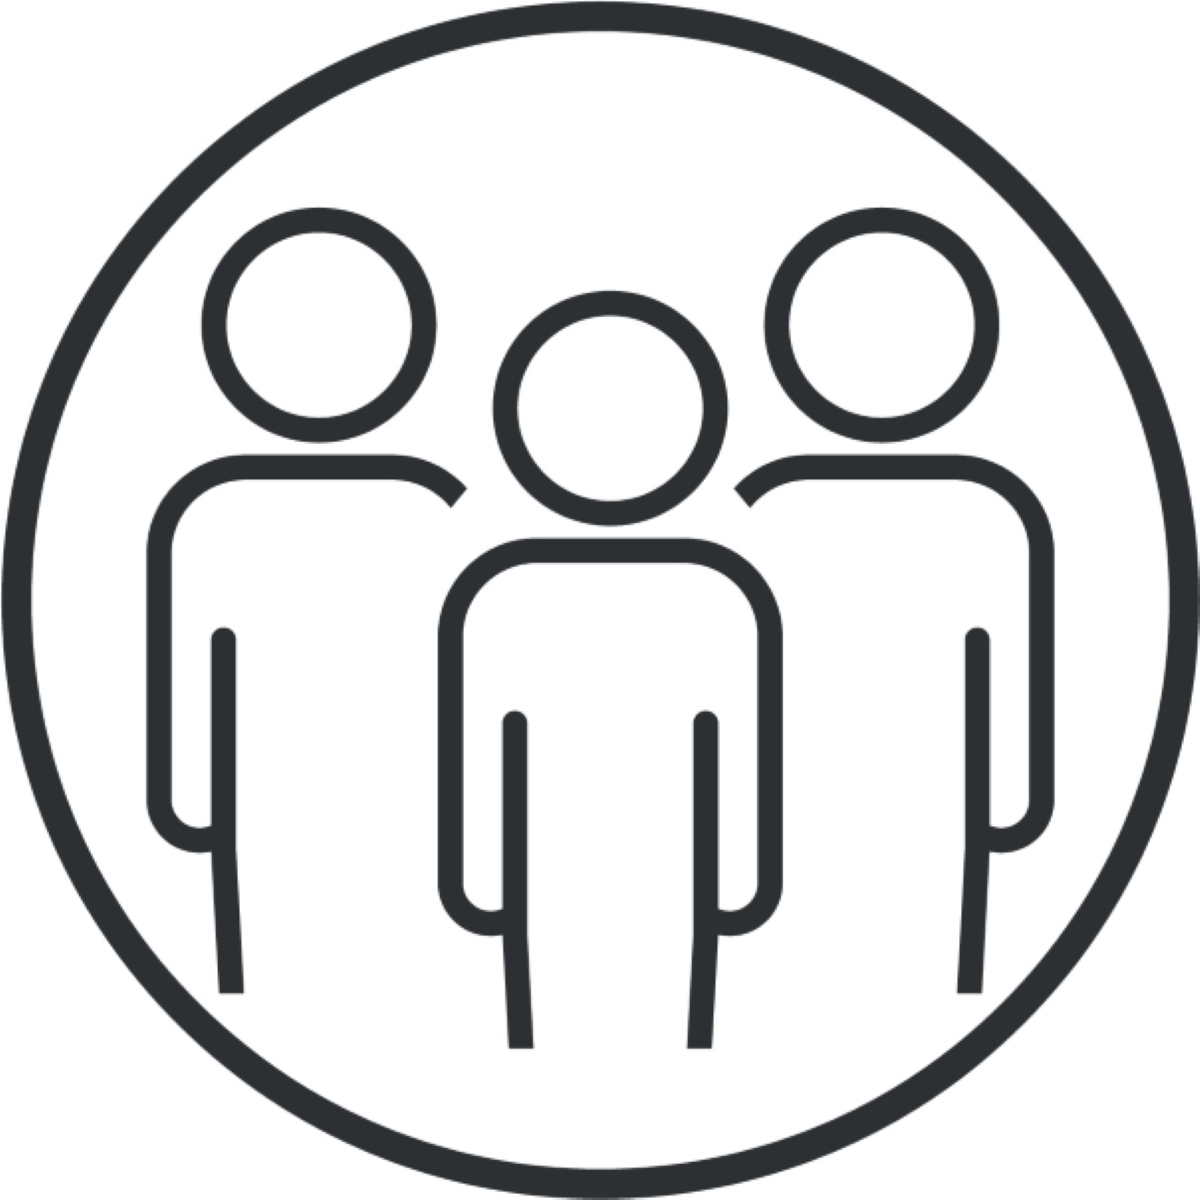
\includegraphics[width=3cm,height=3cm]{ejemplo.jpg}
\end{center}
\vspace*{10mm}
\begin{Large}
\textbf{Desarrollo de una aplicación de control de aforo en Android} \\
\end{Large}
\vspace*{10mm}
\begin{Large}
\textbf{Portiñas} \\
\end{Large}

\vspace*{3in}
\begin{large}
\raggedleft
\textbf{Autores:} Brais Barboza Ordoñez\\
Julián Barcia Facal (julian.bfacal@udc.es) \\
\textbf{Fecha:}\textit{A Coruña, 9 de noviembre de 2021}\\
\textbf{Versión:}\textit{2.0}\\

\end{large}

\end{center}
\end{titlepage} 

\newpage

\addtocontents{toc}{\hspace{-7.5mm} \textbf{Capítulos}}
\addtocontents{toc}{\hfill \textbf{Página} \par}
\addtocontents{toc}{\vspace{-2mm} \hspace{-7.5mm} \hrule \par}

\pagenumbering{empty}

\tableofcontents

\vspace{3cm}

\begin{flushright}
\begin{table}[hbtp]
\begin{center}

\caption{Tabla de versiones.}
\label{tabla:versiones}
\small
\vspace{1ex}

\begin{tabular}{|c|c|l|}
    \hline
    Versión & Fecha & Autor \\
    \hline \hline
    1.0 & 06/10/2021 & Julián y Brais\\ \hline
    2.0 & 09/11/2021 & Julián y Brais\\ \hline
\end{tabular}

\end{center}
\end{table}
\end{flushright}
\newpage
\pagenumbering{arabic}

\section{Introducción}\label{cap.introduccion}

%%
\subsection{Objetivos}
El objetivo principal de este trabajo es gestionar el control de acceso de un edificio o recinto genérico, de tal modo que se tenga un control del número de personas que entran y salen del recinto. Además, buscaremos también crear un lector de identificación, de tal modo que cada usuario pueda ser reconocido de forma individual e inequívoca. De esta manera mediante un teléfono, a través de la app, podremos agilizar los trámites de aforo y acreditación.
%%
\subsection{Motivación}
Debido a la situación de pandemia en la que nos encontramos el control de aforo se ha vuelto un requisito indispensable en muchas ocasiones para poder cumplir las legislaciones continuamente cambiantes. Esta aplicación busca servir, de una manera simplificada, como ayuda para cubrir estas nuevas necesidades que la pandemia ha generado consigo.

%%
\subsection{Trabajo relacionado}
Existe un trabajo fin de grado similar \cite{Safe-Events} que busca proporcionar una aplicación de control de aforo parecida a la nuestra. Sus primeros pasos son fácilmente extrapolables para nuestro cometido y por lo tanto, nos servirá de referencia durante el trabajo.




%%%%%%%
%%%%%%%
\section{Análisis de requisitos}
Esencialmente la aplicación controlará el acceso del personal de un edificio. Con una estación de control en cada acceso, el personal de forma casi transparente podrá acceder al edificio o marcharse del mismo.
El personal contara con un dispositivo con la tecnología NFC (mismamente su teléfono) el cual a la hora de entrar al edificio escanearan contra la aplicación de la puerta, que les garantizara el acceso en caso de cumplir los requisitos necesarios.
%%
\subsection{Funcionalidades}
La aplicación como funcionalidad central tiene el control de aforo de un recinto. Si bien esta idea es bastante simple en un primer momento, la esencia del proyecto reside en su implementación. Sobre un control de aforo clásico como podría ser una persona asignada a llevar la cuenta de la ocupación en una entrada, se proponen una serie de funcionalidades que se implementaran de forma progresiva:
\begin{itemize}
    \item Actualizar el estado (entrada o salida) del sistema mediante dispositivos móviles con tecnología NFC.
    \item Mantener un histórico a disposición de la administración de los accesos y salidas del recinto.
    \item Establecer grupos de personal con franjas horarias de acceso.
    \item Informar al usuario en su dispositivo en caso de que un intento de acceso haya sido denegado.
\end{itemize}

%%
\subsection{Prioridades}
El proyecto tiene como idea central la escalabilidad del mismo. Siendo una idea sencilla permite una alta cantidad de incrementos en función de los requisitos de una organización. Por ello las prioridades serán:
\begin{enumerate}
  \item Conteo de aforo en un único acceso mediante un único terminal de forma manual.
  \item Implementación de un sistema de sincronización entre varios terminales para habilitar el uso en distintos accesos.
  \item Implementación de una aplicación para el acceso mediante dispositivos individuales, permitiendo el control en varios accesos de forma automática
  \item Registro de intentos de acceso y salida.
  \item Posibilidad de crear grupos de usuarios con franjas horarias de acceso.
\end{enumerate}

Cabe destacar que independientemente de las prioridades previamente descritas, el proyecto pretende aumentar de tamaño capa a capa, de forma que cada nivel individual sea plenamente funcional por sí mismo.
%%%%%%%
%%%%%%%
\section{Planificación inicial}

%%
\subsection{Iteraciones}
\begin{enumerate}
    \item Implementar una aplicación que muestre el aforo en el momento actual e incremente o decremente de manera manual, según las personas salgan o entren.
    \item Utilizar NFC \cite{NFC} para ser capaces de identificar a cada persona que entre de manera individual.
    \item Conseguir que este recuento se haga de manera automática al detectar la entrada y salida de usuarios.
    \item Implementar un servidor que actualice los dispositivos de acceso para habilitar el uso simultáneo de varios accesos
    \item Mantener un registro de accesos al registro a nivel individual.
    \item Posibilidad de creación de grupos con franjas horarias de accesos.
\end{enumerate}

%%
\subsection{Responsabilidades}
Considerando que las responsabilidades del proyecto aumentaran de forma exponencial semana a semana, en un primer momento Brais se encargará de actualizar la documentación del proyecto y Julián se encargará de crear el proyecto inicial.
Semana 08/10/2021 - Brais se encargará de la implementación de la tecnología NFC y Julián de implementar la estructura del proyecto.

%%
\subsection{Hitos}
El desarrollo del proyecto se va a organizar en \textit{sprints}, ya que este esquema es el que más se adapta a la idea inicial que tenemos del proyecto.

\begin{itemize}
\item{Fase de planificación: Esta fase se centrará en crear una primera versión del proyecto, diseñando de manera esquemática funcionalidades e interfaz que serán utilizadas próximamente. En esta sección se incluye también la creación de este documento, que será actualizado a lo largo del proyecto}
\item{Fase de desarrollo de la aplicación: Esta fase centra el foco en integrar las funcionalidades y el diseño de la anterior iteración. Al final de esta etapa, se podría un realizar un test para comprobar el correcto funcionamiento de las funciones principales de la aplicación. El test se hará de manera manual, sobre un dispositivo físico, para evitar errores que puede ocultar el emulador.}
\item{Integración del sistema de lectura: Esta sección se focalizará en integrar el método de NFC en las funcionalidades de la aplicación. Al finalizar esta tarea se podría realizar un test para comprobar la correcta lectura y reconocimiento de los dispositivos.}
\item{Implementación del sistema centralizado: Permitir el acceso simultáneo entre varios dispositivos de control, mediante un servidor central.}
\item{Registro de accesos y grupos por franjas horarias: Permitir el acceso a grupos de personal en función de franjas horarias y acceder a registros de acceso.}
\item{Información de la petición en el dispositivo individual: Informar al usuario de si su intento de acceso ha sido aprobado, o de la denegación del mismo con una explicación breve.}
\item{Posibles nuevas funcionalidades y cierre del proyecto: Esta última sección se centrará en añadir nuevas tareas, pero de pequeño tamaño que no pueden comprometer el cierre final del proyecto. Esta última tarea viene acompañada de pruebas sobre el funcionamiento completo de la aplicación.}
\end{itemize}

%%
\subsection{Incidencias}
Si bien la naturaleza del proyecto es simple, se trata de una tecnología desconocida para el equipo de desarrollo. Esto se traducirá probablemente en un aumento de los tiempos de cada tarea.
Sumado a esto, la comunicación NFC puede traer consigo distintas problemáticas, entre ellas la más evidente: se necesitarán varios dispositivos con dicha característica para poder comprobar el funcionamiento del sistema.
Por otra parte, la sincronización de los dispositivos localizados en los accesos del recinto puede resultar complicada, ya que deben ser diseñados sin una interfaz de usuario debido a los requerimientos del proyecto.


%%%%%%%
%%%%%%%
\section{Diseño}
\subsection{Arquitectura}
Se diseñará el proyecto con la arquitectura CLEAN en mente.
Aprovechándonos de la orientación a eventos de Android, implementaremos un modelo vista presentador, donde un evento en el presentador, modificara la vista y llamara al modelo.
En cuanto a la sincronización entre dispositivos, se implementará mediante el uso de un servidor principal con una interfaz API REST.
%%
\subsection{Persistencia}
Guardar en local el estado actual del aforo
Guardar en local el histórico de los accesos
\subsection{Vista}
Nuestro objetivo es la transparencia para el usuario, así que intentaremos mantener una vista simple con pocas opciones, de forma que cometer errores sea más complicado.
\subsection{Comunicaciones}
Entre los dispositivos de acceso y un servidor en la nube como puede ser Firebase.
\subsection{Sensores}
NFC
\subsection{Trabajo en background}
%%%%%%%
%%%%%%%
%% \section{Breve tutorial para trabajar en LaTeX}

\todo[inline]{Breves notas sobre como usar LaTeX  $\rightarrow$ \textbf{eliminar en la versión final} }

Esta es una referencia a un artículo \cite{article-minimal}.

Esta es una referencia a un capítulo dentro de un libro \cite{inbook-minimal}.

Esta es una referencia a un libro \cite{book-minimal}.

Esta es una referencia a un artículo dentro de los proceedings de un congreso \cite{inproceedings-full}.

Esta es una referencia a una url \cite{misc-url}.

\textbf{Esto está escrito en negrita}


\emph{Esto está en enfatizado}

\begin{center}
Este texto está centrado
\end{center}


Esto es una lista:
\begin{itemize}
\item Primer elemento
\item Segundo elemento
\item Lista dentro de otra lista:
	\begin{itemize}
		\item Primer subelemento
		\item Segundo subelemento
	\end{itemize}
\end{itemize}


\section{Título sección}

Esto es una descripción:
\begin{description}
\item[Palabra] descripción de la palabra
\item[Palabra] descripción de la palabra
\end{description}


Y esto una lista numerada:
\begin{enumerate}
\item Elemento
\item Elemento
\item Elemento
\item Elemento
\end{enumerate}


Podemos incluir una figura y referenciarla de esta forma \ref{fig:logo}. Además podemos poner la página en la que está: \pageref{fig:logo}

\begin{figure}[htp]
\begin{center}

\includegraphics[scale=0.2]{figures/udc_old.eps}
\caption{Esta es la etiqueta de la figura}
\label{fig:logo}
\end{center}
\end{figure}


\begin{figure}[htp]
\begin{center}
\framebox{
\includegraphics[scale=0.2]{figures/udc}}
\caption{Esta es la etiqueta de la figura con borde}
\label{fig:logo2}
\end{center}
\end{figure}


\subsection{Título subsección}

Existen varias formas de incluir ecuaciones matemáticas. Las más utilizadas son las siguientes:
\begin{itemize}
 \item Para introducir expresiones matemáticas en el texto, se utiliza como delimitador el símbolo del dólar. Por ejemplo $a \rightarrow b$.
 \item Para introducir ecuaciones matemáticas, se utiliza el entorno \texttt{equation}:
\begin{equation}
 \gamma = \frac{\overline{\alpha}}{\sqrt{\beta}}
\label{eq:equation_example_1}
\end{equation}

\begin{equation}
E(v) =  \int^1_0 \int^1_0 \int^1_0 E_{int}(v(r,s,t)) + E_{ext}(v(r,s,t))drdsdt 
\label{eq:equation_example_2}
\end{equation}	
Un subíndice se especifica con el guión bajo y un superíndice con el circunflejo. Si el super/subíndice contiene varios caracteres, estos deben estar delimitados por llaves. Consultar el manual para comprobar como se pueden introducir símbolos y expresiones matemáticas en latex.
\end{itemize}



\subsection{Título subsección}

Esto es una subsección\footnote{Así se hace una nota a pie de página}.


Así introducimos texto sin ningún tipo de formato latex:
\begin{verbatim}
  4 drwxr-xr-x  2 noelia imagen   4096 2005-09-12 12:09 figures
  4 -rwxr--r--  1 noelia imagen    585 2005-09-12 16:56 Makefile
  4 -rw-r--r--  1 noelia imagen    647 2005-09-12 17:38 memoria.aux
  4 -rw-r--r--  1 noelia imagen   1011 2005-09-12 17:18 memoria.bbl
  4 -rw-r--r--  1 noelia imagen   1171 2005-09-12 17:18 memoria.blg
 16 -rw-r--r--  1 noelia imagen  13440 2005-09-12 17:38 memoria.dvi
  4 -rw-r--r--  1 noelia imagen    412 2005-09-12 17:38 memoria.glg
  4 -rw-r--r--  1 noelia imagen    188 2005-09-12 17:38 memoria.glo
  4 -rw-r--r--  1 noelia imagen    241 2005-09-12 17:38 memoria.gls
  4 -rw-r--r--  1 noelia imagen    299 2005-09-12 17:38 memoria.ist
  4 -rw-r--r--  1 noelia imagen    283 2005-09-12 17:38 memoria.lof
 12 -rw-r--r--  1 noelia imagen   8997 2005-09-12 17:38 memoria.log
  4 -rw-r--r--  1 noelia imagen     87 2005-09-12 17:38 memoria.lot
108 -rw-r--r--  1 noelia imagen 103492 2005-09-12 17:18 memoria.pdf
280 -rw-r--r--  1 noelia imagen 278687 2005-09-12 17:18 memoria.ps
  4 -rwxr--r--  1 noelia imagen   1887 2005-09-12 17:40 memoria.tex
  4 -rw-r--r--  1 noelia imagen    735 2005-09-12 17:38 memoria.toc
\end{verbatim}



\subsubsection{Título subsubsección}

La figura \ref{tab:tabla_ejemplo} muestra un ejemplo de tabla básica. Para crear una tabla se utiliza el entorno \texttt{tabular} dentro del flotante \texttt{table}. 

%% PARA ENTENDER ESTE TEXTO, MEJOR COMPILAR Y LEER EL DVI/PS/PDF
%% \ es un caracter reservado de latex por lo que para poder utilizarlo cuando escribimos debemos utilizar el comando \textbackslash
%% &, {, } también son caracteres reservados. En este caso, para escribirlos en el texto, anteponemos \ al caracter

Tras \texttt{\textbackslash begin\{tabular\}} se declara el número de columnas de la tabla. Cada columna se especifica con una letra:
\begin{description}
 \item [c] Si el texto en la columna está centrado
 \item [l] Si el texto en la columna está alineado a la izquierda
 \item [r] Si el texto en la columna está alineado a la derecha
\end{description}

\begin{table}[htp]
\caption{Tabla de ejemplo}
\label{tab:tabla_ejemplo}
\begin{center}
 \begin{tabular}{rlc}\hline
  Fila 1 Col. 1 larálala & Fila 1 Col. 2 lara & Fila 1 Col. 3  lalalalalalalala\\ \hline
  Fila 2 Col. 1 & Fila 2 Col. 2 & Fila 2 Col. 3 \\ \hline
 \end{tabular}
\end{center}
\end{table}

Así \texttt{\textbackslash begin\{tabular\}\{rrrr\}} indica 4 columnas con texto alineado a la derecha y \texttt{\textbackslash begin\{tabular\}\{cl\}} indica dos columnas, la primera centrada y la segunda alineada a la izquierda.

Entre \texttt{\textbackslash begin\{tabular\}\{\ldots\}} y \texttt{\textbackslash end\{tabular\}} se escribe el contenido de la tabla. Las columnas se separan con \& y las filas con \textbackslash \textbackslash. Un ejemplo de una fila con tres columnas sería el siguiente:
\begin{center}
 \texttt{ aaa \& bbbb \& cccc \textbackslash \textbackslash}\footnote{Importante: debe coincidir el número de columnas en la declaración con el número de columnas que se escriben dentro de la tabla}. 
\end{center}

Para incluir lineas horizontales existe el comando \texttt{\textbackslash hline}. Tras \texttt{\textbackslash begin\{tabular\}\{\ldots\}} podemos incluir un \texttt{\textbackslash hline}, pero \textbf{ojo}, en cada fila \texttt{\textbackslash hline} siempre debe ir tras \textbackslash \textbackslash.

También es posible incluir líneas verticales, pero los manuales de estilo no lo aconsejan. Las líneas verticales se definen en la declaración con barras verticales. Por ejemplo, con \{\textbar c  \textbar c \textbar c\}  se crearían 3 líneas verticales, una antes de la primera columna, otra entre la primera y la segunda columna, y la tercera, entre la segunda y tercera columna.

Dentro de las tablas podemos incluir expresiones matemáticas, texto enfatizado, negrita, etc. Es posible también fusionar varias filas o varias columnas dentro de una misma tabla. Para ello, consultar en manuales los comandos/paquetes \texttt{multirow} y \texttt{multicol}.


Nueva referencia \cite{milibro}.





\bibliographystyle{pfc-fic}
\bibliography{biblio}
\addcontentsline{toc}{section}{Bibliografía}

\end{document}
